\chapter{Readout Experiment}\label{chap:readout}
With the knowledge of how readout are carried out, we are now ready to take on the actual readout process. In this chapter, we will be performing the analysis of a readout process from the laboratory to determine how good it is.

\section{Experimental Setup}
While most of the work in this thesis will be theoretical and computational, we will try to understand, calibrate and model a physical system. This section will serve as a short overview of the setup.
% \todo{Write this section properly.}

\subsection{Soprano Chip}
The experiments are run on the Soprano 6 qubit Chip on qubit ? (see figure \ref{fig:soprano}), a flux tuneable transmon connected to a resonator, drive line and flux line to tune the transmon. The resonator is connected to a feed line which is further connected to the five other resonators (some through a Purcell filter).

\begin{figure}[h]
    \begin{minipage}{0.50\textwidth}
        \centering
        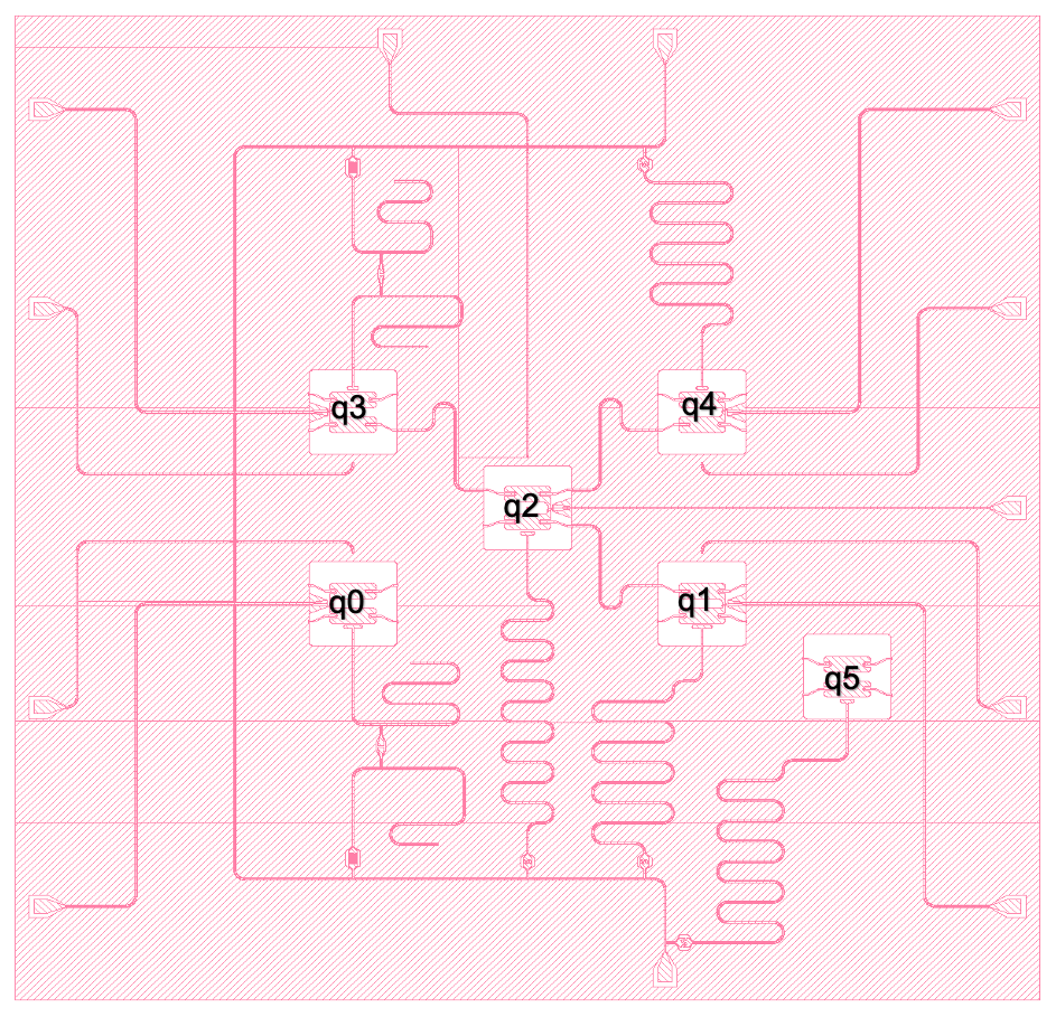
\includegraphics[height = 5 cm]{Figs/hardware/layout.png}
    \end{minipage}
        \begin{minipage}{0.50\textwidth}
        \centering
        \includegraphics[height = 5 cm]{Figs/hardware/layout_photo.png}
    \end{minipage}
    \caption{The Soprano Chip layout and a picture.}
    \label{fig:soprano}
\end{figure}

\subsection{Control Hardware}
In order to control the qubit and resonator, an arbitrary waveform generator and processing device is used. In this experiment, this is done with an OPX \cite{noauthor_opx_nodate}. The OPX outputs two signals to drive the qubit and one to the readout line. It has an envelope resolution of 1 GS/s and can process waves with a frequency of 400 MHz. In addition, it is connected with two channels for incoming signal from the readout line which can be demodulated on the onboard FPGA chip. 

Since the signal needed for qubit and resonator control is of order 5-10 GHz, another device for up- and downconversion is needed. Here, we make use of the Octave \cite{noauthor_octave_nodate}. The Octave has multiple local oscillators for down converting signal one of which support up conversion as well. This one is used for readout, and one of the others are used for qubit control. All signal support IQ mixibng interal IQ mixers allowing us to split the signal. 

The two devices can be controlled by using accessing an API using Python. For this thesis the higher level module OPX\_Control was used which simplifies writing and running experiment using the OPX and Octave. 

In addition to the driving lines, a DC line is also coupled directly from the OPX to the fridge to adjust the flux in the qubit. This will be constant for all experiments in the qubit sweet spot, so it will mostly be forgotten. 

\subsection{Cooling and Amplifiation}
To keep the soprano chip cold, it is places in a Cryostate capable of cooling to $\approx 30 \text{mK}$ while keeping the chip in vaccum to reduce thermal fluctuations and interactions with the environment. 

\begin{itemize}
    \item Down Conversion Line
    \item Up Conversion Line -> TWPA -> higher temperature amplifiers 
\end{itemize}



\begin{figure}
    \centering
    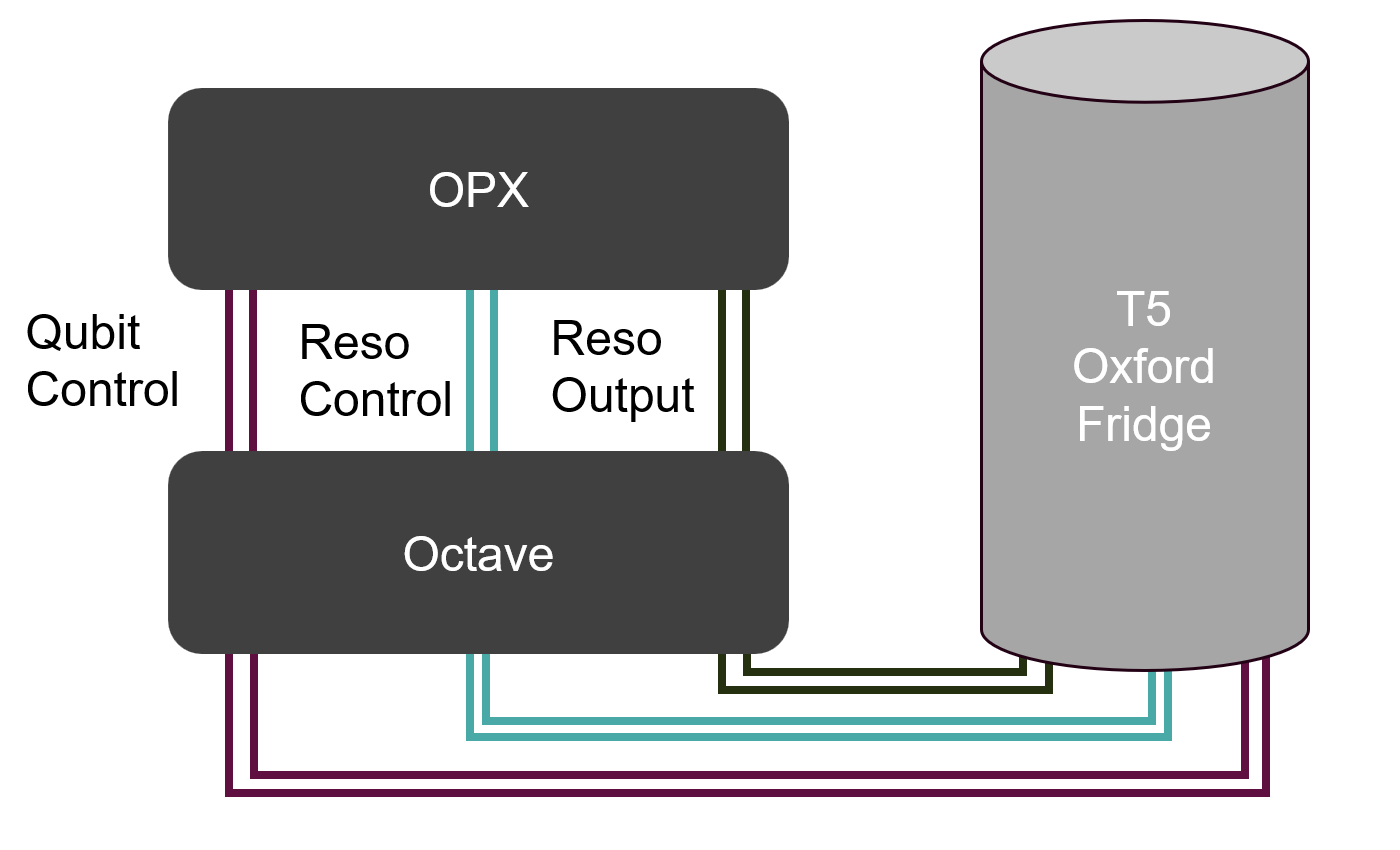
\includegraphics[width=1\linewidth]{Figs//hardware/Setup.png}
    \caption{A crude schematic of the setup. Qubit control and resonator lines are sent through the octave where they are up converted before going to T5. In the other direction, the signal is downconverted and mixed in the IQ mixer before reentering the OPX where it gets demodulated.}
    \label{fig:enter-label}
\end{figure}


\section{Readout Fidelity}
First, we need to define a goodness measure for the readout. As a start, we formulate the goal of the readout process as following:
\begin{itemize}
    \item Given a quantum state $\rho$ a readout is a scheme that predicts a state $\sigma$, such that $\sigma$ is on average as close to $\rho$ as possible.
\end{itemize}
While this is a bit easier to work with, we still need to find a quantity for "closeness" between a density matrix and our prediction. Mathematically, we can achieve this by defining a formal distance, such as the trace-norm on the vector space of $2\times2$ matrices: $\mathcal{M}^2$ \cite{wilde_classical_2016}:
\begin{equation}
    ||\rho - \sigma|| = \Tr \left[\sqrt{\left(\rho - \sigma \right)^\dagger \left(\rho - \sigma \right)} \right]
\end{equation}
which has the desired properties like being $||\rho_{\text{pred}} - \rho_{\text{true}}|| = 0$, if our prediction is correct. While the trace-norm is an excellent tool, often a related quantity will be used in quantum physics.  We instead use the fidelity, which has a general form defined by:
\begin{equation}
    F(\sigma, \rho) = \left(\Tr\sqrt{\sqrt{\rho} \sigma \sqrt{\rho}}\right)^2
\end{equation}
Here $\sqrt{\rho}$ is the matrix, which satisfies $(\sqrt{\rho})^2 \rho$. The relation to the trace norm is by bounds of the Fidelity \footnote{both upper and lower bound by $1 - \sqrt{F(\rho, \sigma)} \leq \frac{1}{2} ||\rho - \sigma|| \leq \sqrt{1 - F(\rho, \sigma)}$ \cite{wilde_classical_2016}}.  In addition, it has other nice properties: it is symmetric in $\sigma \leftrightarrow \rho$ and it reduce significantly if one of the states are pure. In our schemes the readout will always predict pure state of either $\ket{1}\bra{1}$ or $\ket{0}\bra{0}$. In this case $\sigma = \ket{k}\bra{k}$ and the full equation can be written as:
\begin{align*}
    F(\sigma, \rho) = F(\rho, \sigma) &= \left(\Tr\sqrt{\sqrt{\sigma} \rho \sqrt{\sigma}}\right)^2 \\
    &= \Big(\Tr \left(\ket{k}\mel{k}{\rho}{k}\bra{k}\right)\Big)^2\\
    &= \mel{k}{\rho}{k}
\end{align*}
Because of the stochastic nature of quantum mechanics, estimating this quantity takes multiple measurements. We repeat it $N$ times and take the average over the process.  
\begin{equation}
    \mathbf{E}\left[F(\sigma, \rho)\right] = \frac{1}{N}\sum_i^N F(\sigma_i, \rho_i)
\end{equation}
In the full readout scheme, we should be able to properly measure both $\rho = \ket{1}\bra{1}$ and $\ket{0}\bra{0}$. For this reason, we also average over the initialization of the qubit. 
\begin{equation}
     \frac12 \left(\mathbf{E}\left[F(\sigma(\rho_0), \rho_0)\right] +  \mathbf{E}\left[F(\sigma(\rho_1), \rho_1)\right]\right)
\end{equation}
Here $\rho_k$ refers to the best initialization of $\ket{k}\bra{k}$, we can make and $\sigma(\rho_i)$ the prediction our readout scheme produces given that state. It is important to note, that if we are not capable of initializing the qubit in a desired pure state\footnote{which we are not}, the initialization and the readout of the initialization are both contributors to the fidelity measure. Together these two factor are referred to as the State Preparation and Measurement errors or SPAM for short.

One drawback of this fidelity scheme is that it is $\frac12$ for a completely random classification\footnote{And a classification scheme with $F<\frac12$ can be better by just swapping the output labels}. For this reason, most definitions of the SPAM fidelity \cite{gambetta_protocols_2007, blais_circuit_2021} is re-scaled such that the fidelity score lies between $0$ and $1$:
\begin{equation}
    F_{\text{SPAM}} = \mathbf{E}[F(\sigma(\rho_1), \rho_1)] + \mathbf{E}[F(\sigma(\rho_0), \rho_0)] - 1
\end{equation}
Which is the definition we will be using to define the "goodness" of a readout (and initialization, which will be implicit if nothing else is mentioned). Over many repetetions and with pure state predictions, the expectation value of the fidelity, can be found by probability of classifying correctly:
\begin{equation}
     \mathbf{E}[F(\sigma(\rho_k), \rho_k)] = P(\text{ro} = "k"| \text{ init} = k)
\end{equation}
where "ro" is short for readout and "init" for initialization. Or writing it in terms of the infidelities $ P(\text{ro} = "0"| \text{ init} = 0) = 1 - P(\text{ro} = "1"| \text{ init} = 0)$, we get the estimate as:
\begin{equation}\label{eq:fidelity_spam_estimate}
    F_{\text{SPAM}} = 1 - P(\text{ro} = "0"| \text{ init} = 1) - P(\text{ro} = "1"| \text{ init} = 0)  
\end{equation}




\section{Determining the Readout Fidelity}
We will now what we are learned into a scheme for determining the readout fidelity of our superconducting qubit. The scheme is visualized in figure \ref{fig:circuit_qubit_readout_test} and goes as:
\begin{marginfigure}
    \centering
    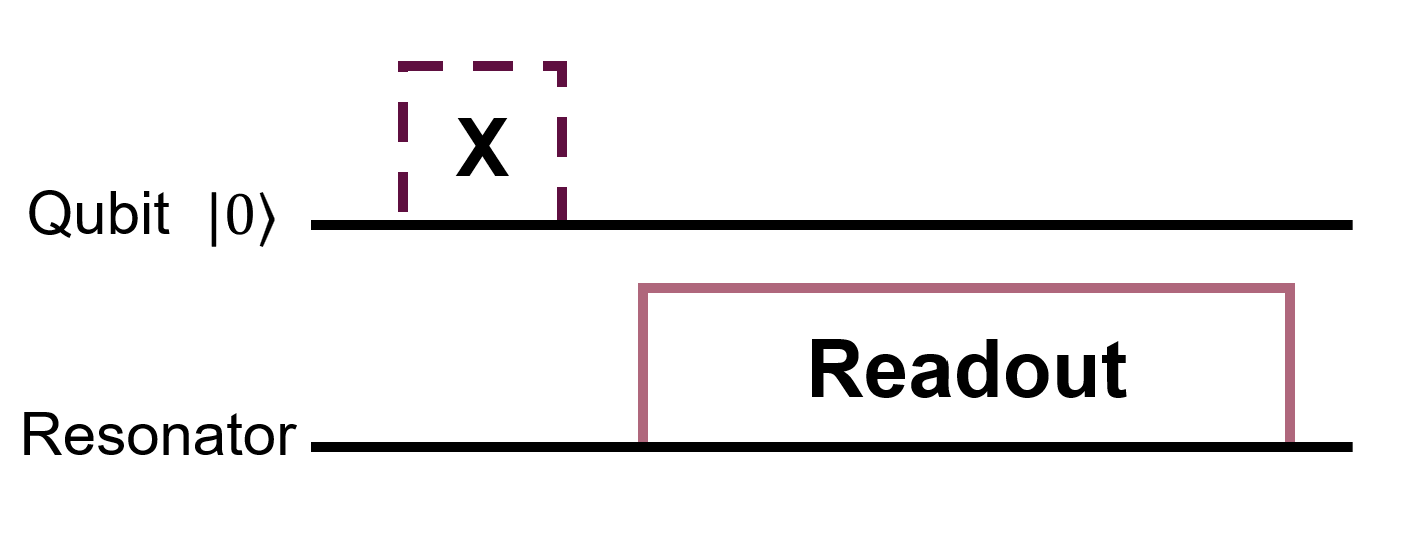
\includegraphics[]{Figs/circuits/readout_test.png}
    \caption{Circuit displaying the process of making a readout test. In half the initialization, an $X$ gate is applied to excite the qubit to $\ket{1}$. This is followed by a readout pulse on the resonator.}
    \label{fig:circuit_qubit_readout_test}
\end{marginfigure}
\begin{enumerate}
    \item The Qubit is initialized by waiting a duration of 10 (5?) times the $T_1$ such that it is in its equilibrium state. This will be the initilization $\rho_0$.
    \item In half the experiments, we apply an $X_\pi$ pulse, to excite the qubit into the first excited state. This gives us our $\rho_1$.
    \item We now apply a square\footnote{We have a 10 $ns$ ramp-up and ramp-down period to avoid "kicking" the system". This is neglected in our analysis and later in simulations} resonator pulse at frequency $f_d = f_r$ (in between the two states shift) lasting $600 \text{ns}$. This starts movement in the IQ plane  analogous to what was described in section \ref{sec:resonator_decays}. The feed line output signal is monitored using a hetereodyne measurement-scheme which we described in section \ref{sec:heterodyne_measurement}. This leads to I and Q signal which is tracked digitized every $ns$ and stored for post processing.
    \item Steps 1-3 is repeated 1000 times for intialization $0$ and for initialization $1$.
\end{enumerate}
In the post processing (which is visualized in the top row of figure \ref{fig:readout_process}), we have the initialization label and the I and Q trajectories of the readout pulse. By demodulating them at the intermediate frequency and integrating the signal we arrive at one value set for $(I, Q)$. Plotting the distribution of our, we can find the projection line with the largest separation using Linear Discriminant Analysis. This is done by using the implementation in SKLearn \cite{Pedregosa_sklearn}. This allows us to project all points onto the axis resulting in a 1D histogram. At every value on this axis, we can calculate the fidelity by:
 By picking the threshhold which maximized the fidelity, we have a measure for the fidelity of this readout protocol. In our experiment this lead to the fidelity.
\begin{equation}
    F_{\text{SPAM}} = 0.613\pm 0.018
\end{equation}
It is worth noting that this is not the best optimized readout signal, we can achieve. The amplitude of the resonator pulse is here lower than optimal. The goal is however not to do optimal readout but instead study the contribution to the SPAM infidelity, and a stronger pulse would require a bigger Hilbert space in our simulations. We will return to this challenge later.
\begin{figure*}[t]
    \centering
    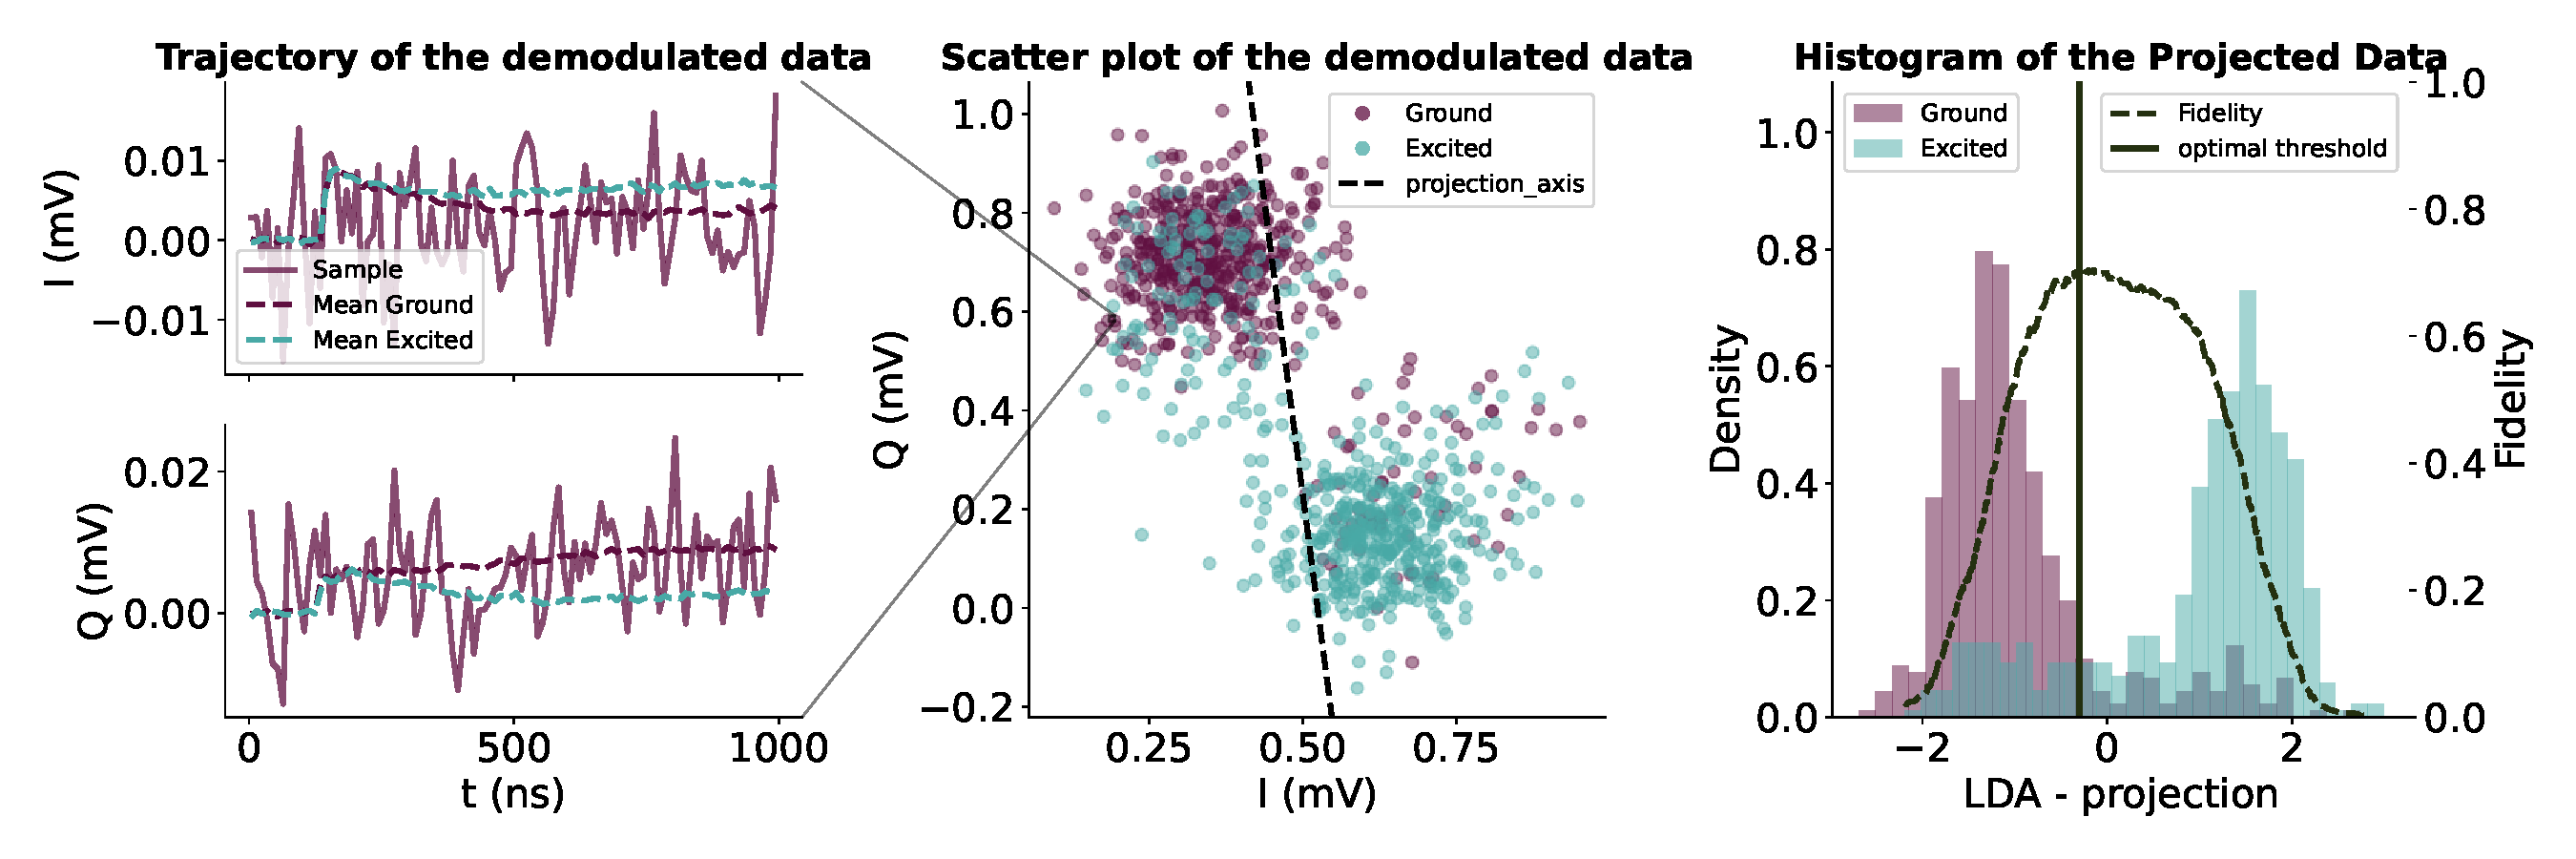
\includegraphics{Readout/Figs/Introduction.pdf}
    % 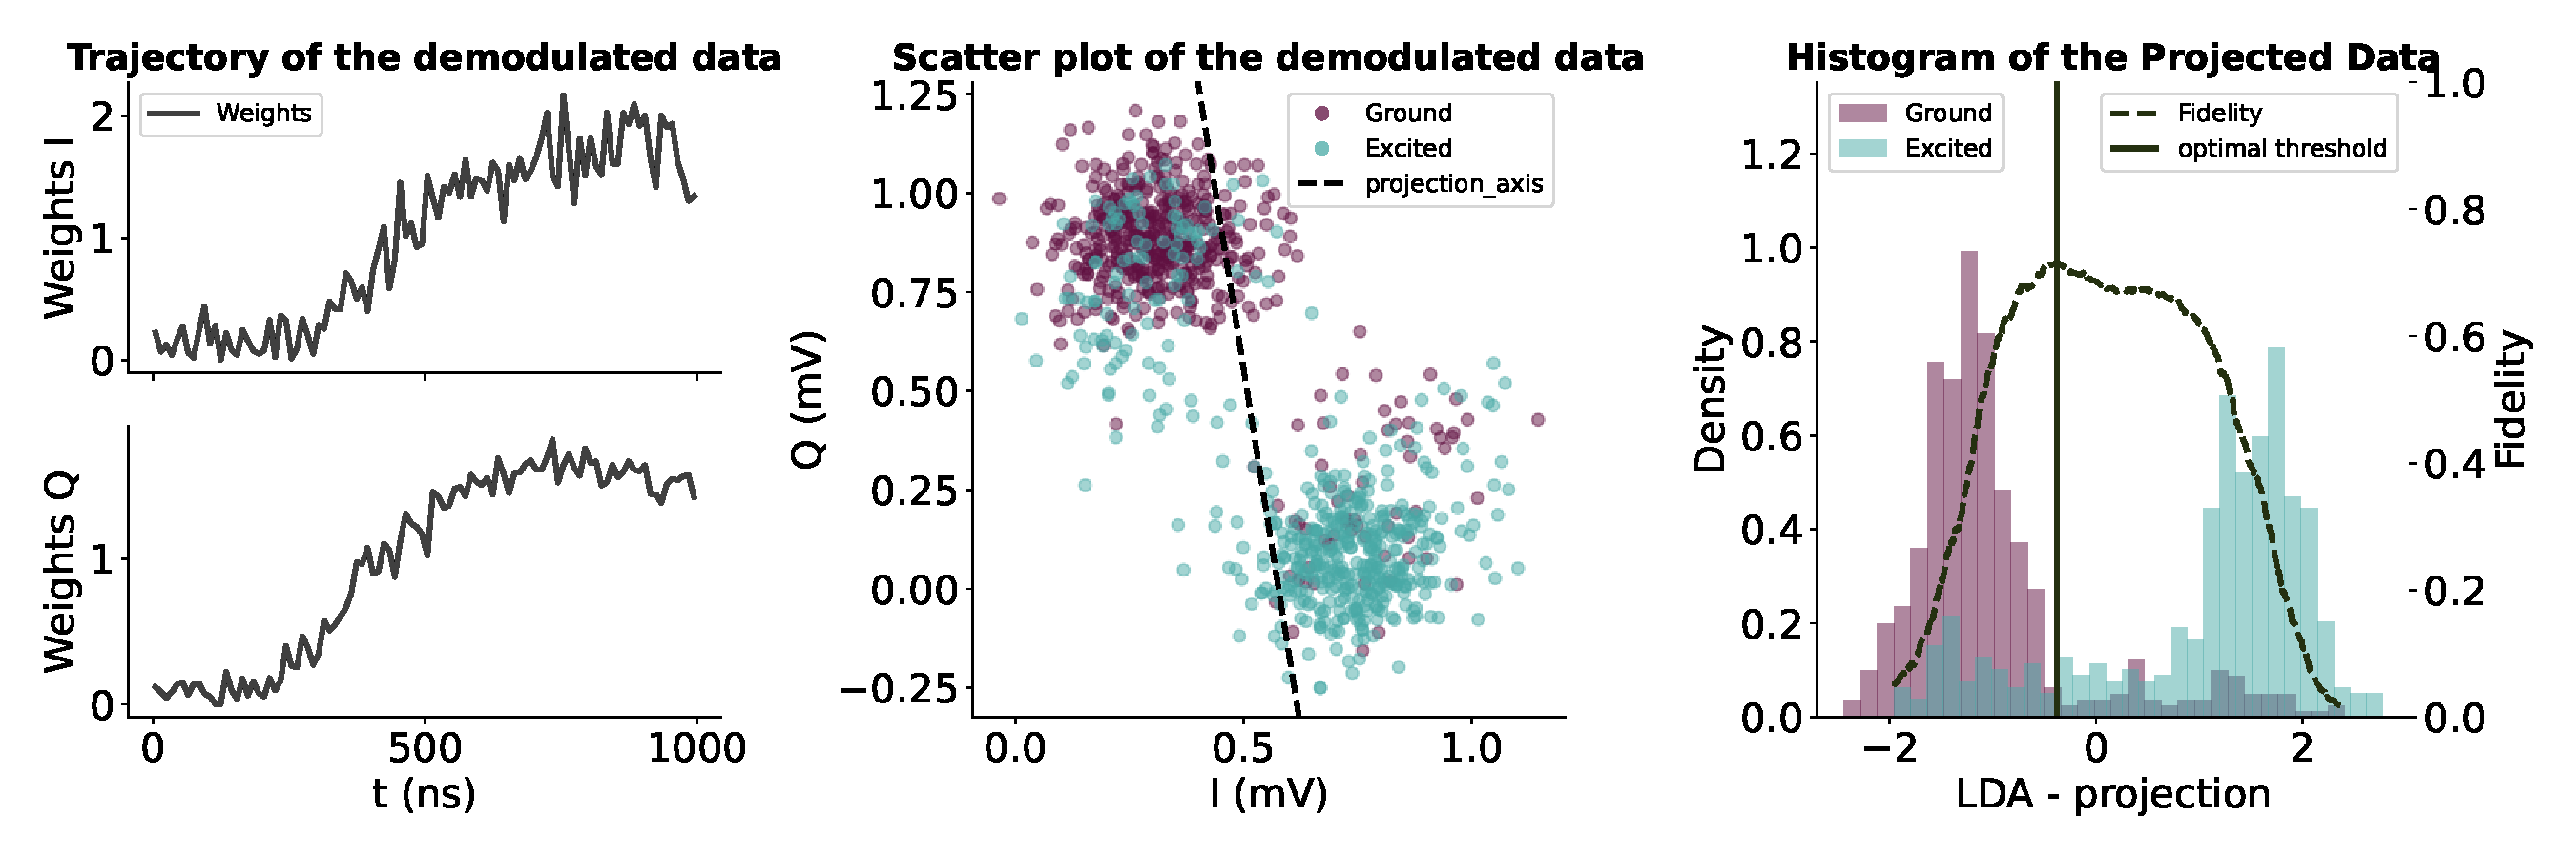
\includegraphics{Readout/Figs/Weighted.pdf}
    \caption{Visualization of the Fidelity calculation for no weights (top) and optimal weights (bottom). The top left panel shows an example trajectory along with the mean trajectories. While the bottom left panel are the optimal weights calculated to separate the two distributions. The middle panels are the IQ distributions shown in scatter plots. In the right panels the IQ distributions are projected unto the axis with the biggest separation. Here the Fidelity as a function of threshold is plotted and the optimal is marked.}
    % \label{fig:simple_weights_fidelty}
    \label{fig:readout_process}
\end{figure*}



% Given a set of IQ measurement of the qubit initialized in $\ket{0}$ and $\ket{1}$ respectively, we want to combine it to maximize the separation between the $\ket{0}$ and $\ket{1}$ state. If the resonator has reached its steady state and the measurements come from a Gaussian distribution, it is sufficient to sum/mean the whole trace, and compare the final distributions. Under this assumption we will get a distribution of IQ values. 

% We now pick the projection line through this plane that best separates the $\ket{0}$ and $\ket{1}$ group. This can for example be done by using an Linear Discriminant Analysis\footnote{Given two dimensional labels and data in multiple dimensions, it finds the axis with biggest separation. Here we have used the implementation from sklearn. \cite{sklearn}}. On this axis, we can now set a threshold. If we set it such that the fidelity is maximized, we have defined our simple readout scheme. The process can be see in the top row in figure \ref{fig:readout_process}.


\section{Filtering and Weights}
Summing the points to get a better classification works well if the points are from a steady distribution, as they are in the steady state. In reality however, we might have different other attributes in the readout signal, that we want to weigh differently. A typical example, is that the qubit ramp-up interval will have less separation than in the steady state. Further, the qubit will also experiment energy decay from $\ket{1}\to \ket{0}$\footnote{Or absorb energy to go the other way} or we might even want to include signal during resonator depletion. A solution to this is by weighing the signal at different times. 

\subsection{Weighting of the Input}
Under the assumption that the measured signal from the resonator will be Gaussian in the IQ plane, the points at different times are uncorrelated and symmetric \cite{magesan_machine_2015}  it is possible to derive optimal linear weights. To do this, we first allow for a weighting parameters at each time step in each quadrature. The signal takes the form of $\sum_{x = I, Q}\sum_t k_{x, t} \cdot x_t$. And defining the signal as the difference between the signal from $\ket{0}$ and $\ket{1}$ we have:
\begin{equation}
    \Delta S = \sum_X \sum_t k_{x, t} (\expval{X_0 - X_1} + \xi_t)
\end{equation}
Where we have collected the noise terms from both trajectories into one parameter $\xi_t$. The Signal to Noise Ratio ($\SNR$) is defined by: %To maximize the Signal to Noise Ratio defined by the signal strength divided with the variance we find the mean and variance of the separated signal as:
\begin{equation}
    \SNR^2 = \frac{|\expval{\Delta S}|^2}{\Var(\Delta S)} 
\end{equation}
where we can find the mean and variance of the signal as:
\begin{align}
    \expval{\Delta S} &= \sum_X \sum_t k_{x, t} (\expval{X_0 - X_1} \\
    \Var(\Delta S) &= \sum_X \sum_t k_{x, t}^2 \left( \Var(\expval{X_0 - X_1}) + \Var(\xi) \right)
\end{align}
The SNR can be maximized by differentiating with respect to the weights and setting the derivative equal to $0$: $\partial / \partial k_{x, t} \SNR = 0$. The weights that maximize the signal is found by  setting:
\begin{equation}
    k_{x, t} = \frac{\expval{X_0 - X_1}}{\Var(\Delta S)}
\end{equation}
Where we will determine the variance and average expected difference experimentally by performing a set of measurement and calculating the mean difference and variance to determine the weights \cite{ryan_tomography_2015}.

In the lower row in figure \ref{fig:readout_process} the experiment is repeated but with calculated linear weights before rotating. As we can see the readout fidelity is now:
\begin{equation}
    F_{\text{readout}} = 0.620 \pm 0.017
\end{equation}
This is very close to readout fidelity of the simple weights. While it appears that these weights are only a marginal improvement, we should still notice that the two IQ distributions become narrower. In quantifying this, we can calculate the Signal to Noise ratio for the two example. We see that $\SNR = 2.54$ goes to $\SNR = 2.19$ when we apply the weights. This corresponds to reduce the overlap from the distributions from $1.43\%$ to $0.55\%$. With 2000 samples (1000 $\ket{0}$ and 1000 $\ket{1}$), we would win around 10-20 additional correct classifications\footnote{In the actual experiment, we find 7, but this is subject to some randomness and still a lot smaller than the uncertainties.}, but if the distributions were to be closer, the increase in SNR by $0.25$ would have had an even bigger impact on the fidelity.


\subsection{Non-Linear Classification Schemes ** }
The classification scheme above is very common, since it can be combined with the demodulation (both linear operation) and is able to be run in most FPGA processers like the one installed in the OPX control in our laboratory. This allows for fast executions and easy to calibration. However, the assumptions for assumption are not entirely realistic. 

One example is in a relaxation during the readout. If the qubit state halfway through changes from $\ket{1}\to \ket{0}$ our measurement record will then start to follow the trajectory of the ground state. In this case, we should weigh the points differently depending on the information provided by the rest of the trajectories. We can do such a generalization either by allowing for a covariant weights\cite{gambetta_protocols_2007} or by applying machine learning methods like neural networks \cite{lienhard_deep-neural-network_2022}.

% This becomes very clear, when we think about the effects of $T_1$ which splits ... \todo{Is $T_1$ a good example? What else do we violate}. One could setup allow for covariance between measurements or nonlinear kernels. Or a different method is to use Machine Learning methods to distinguish the trajectories. This allows for the possibility of weighting the inputs differently depending on the beginning of the signal beyond the average behaviour.\todo{Do we want to try this quick? Otherwise, we can reduce this to a comment in the above section.}



\section{Postselection}\label{sec:postselection}
In some instances, we do not mind running with a large overhead in order to increase our readout fidelity. In these cases, we can instead associate a probability of a given trajectory belonging to the $0$ or $1$ group and then pick the fraction $f$ with the most certain classifications. Since $T_1$ decay tends to happen somewhere during the measurement, the points will often be placed in some tail going from $1 \to 0$. Furthermore, the overlap between the two distributions will be in between them. So by sacrificing the middle points, the leftover errors are mainly due to inseparable distributions. 

Wrong initialization gives a mixed state, which will lead to a part of the distribution identitical to the other initialization. For this reason, the state initialization fidelity can be cruedly approximated by taking the fidelity from SPAM in the limit where $f\to 0$. In figure \ref{fig:postselection_plot}, we have done this post selection with the samples used in figure \ref{fig:readout_process}. By fitting a polynomial, here 3rd order, we can approximate the limit for the fraction of data going to 0 as:
\begin{equation}
    F_{\text{init}} \approx \lim_{f \to 0} F_{\text{SPAM}} = 0.82 \pm 0.02
\end{equation}
which should not be taken as a direct measure, but more one that we can return to in a discussion after some more work.\todo{Return to this statistic at some point to conclude.}


\begin{figure}[t]
    \centering
    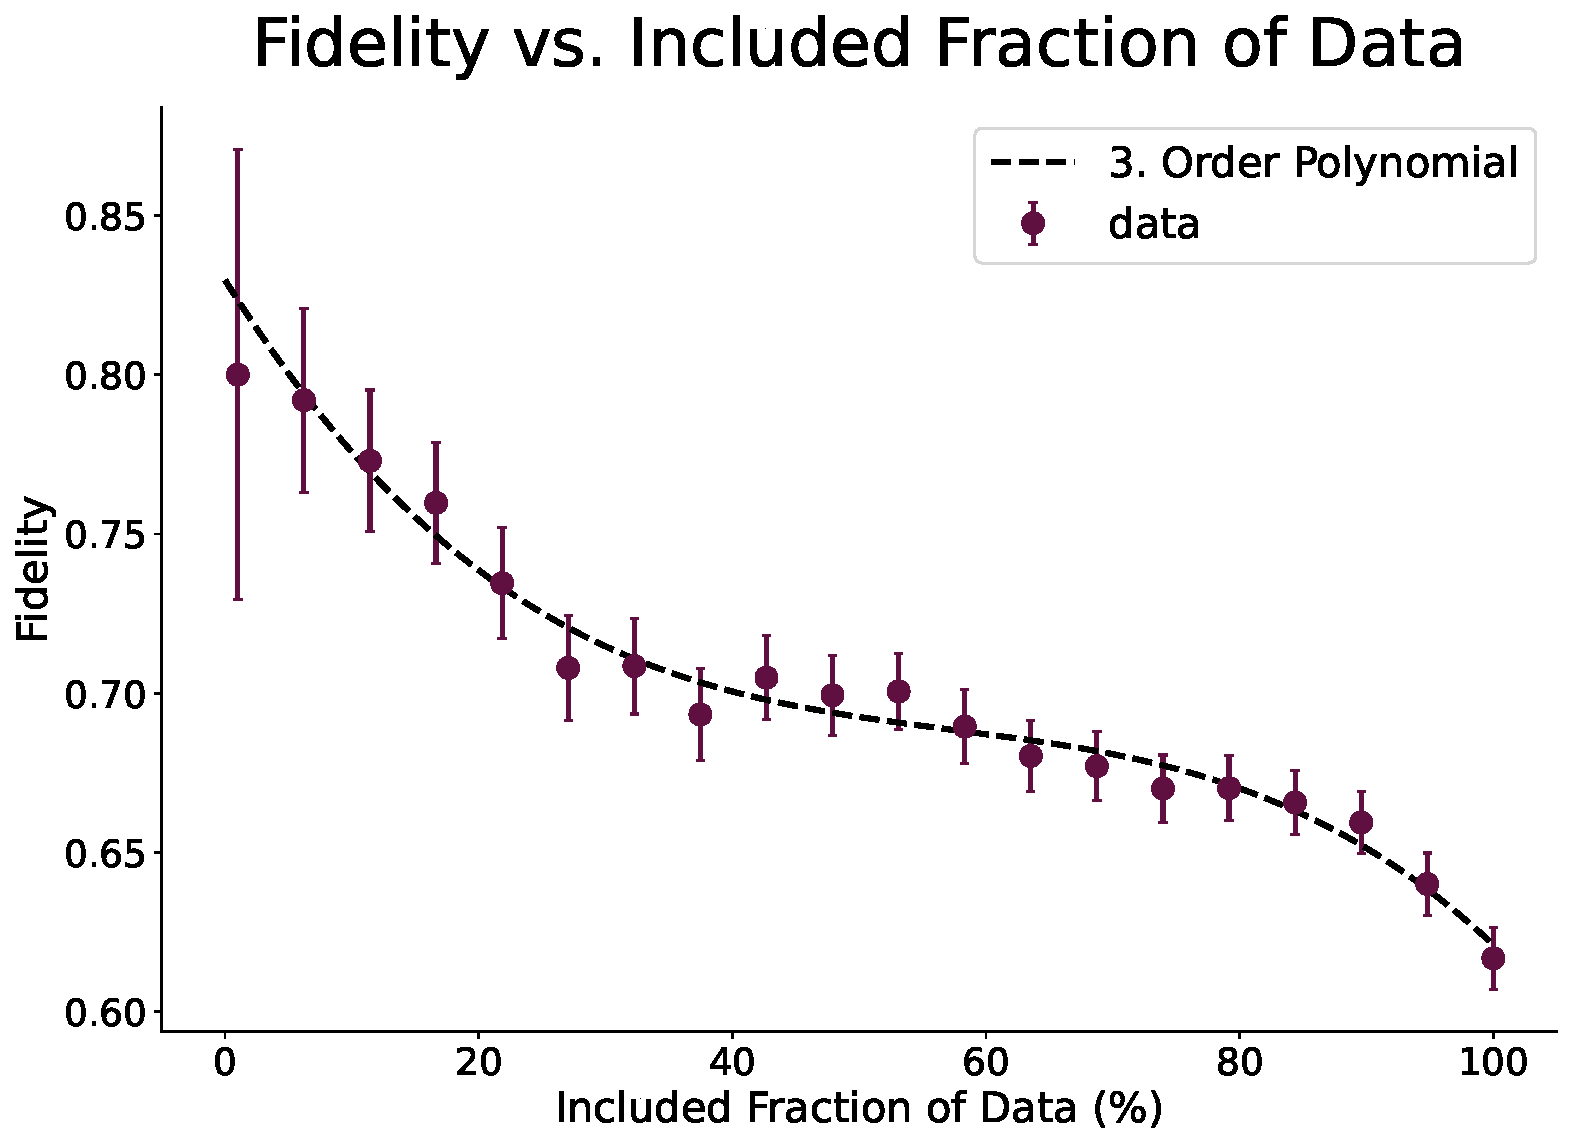
\includegraphics[]{Readout/Figs/fidelity_vs_included_fraction.pdf}
    \caption{The Fidelity of an initialize and measure experiment depending on the fraction of most certain points, we include. The curve is fitted with a second order polynomial to estimate the limit for the fraction going to $0$.}
    \label{fig:postselection_plot}
\end{figure}

% The following sections are also possible:
% \begin{itemize}
%     \item Adjusting Pulse Parameters
%     \item Strategies
%     \item Counter Depopulation Pulse
% \end{itemize}

% \section{Adjusting Pulse Parameters*}
% \begin{itemize}
%     \item Reading out after, since we have to wait for depopulation anyways.
% \end{itemize}

% \section{Strategies*}
% \begin{itemize}
%     \item This can be kicking the qubit with a $\pi_{12}$ pulse. 
% \end{itemize}

% \section{Counter Depopulation Pulse*}
% \begin{itemize}
%     \item Stimulated depopulation
% \end{itemize}